\section{时间隐通道构建方法}
\label{chap:backinfo:ctc}

%概述,在以太网中进行时间隐通道的研究已经有成果
基于网络的时间隐通道,是隐通道研究中一个重要的课题。随着IP网络的发展,基于单主机的时间隐通道,已经难以满足隐蔽传输需求。借助IP网络高带宽、大流量的优势,基于IP网络的时间隐通道在传输性能、隐蔽性方面有了进一步提升。
%在移动互联网下的方案,也已经存在
当前移动互联网已经成为主流,面向移动终端的流媒体应用及实时通信应用兴起,为时间隐通道提供了新的平台。
%这些方案中有一些通用的方法及保证鲁棒性的策略
时间隐通道面对一个共同难题,是如何在噪声干扰下保证传输鲁棒性。作为寄生信道,时间隐通道与宿主信道在信噪比方面有较大差距,在方法设计和优化中需要针对性改进。

\subsection{适于以太网的时间隐通道构建方法}
\label{chap:backinfo:ctc:ethernet}
%经典时间隐通道
%IPD-CTC
适于以太网的时间隐通道,通常调整时间间隔或数据包序号,实现隐蔽消息传输。由于时间隐通道与检测方法是对应的,如果时间隐通道利用了未公开的传输特征,则检测方法的识别率较低。

\insertFigure{
	\begin{figure}[htbp]
		\centering
        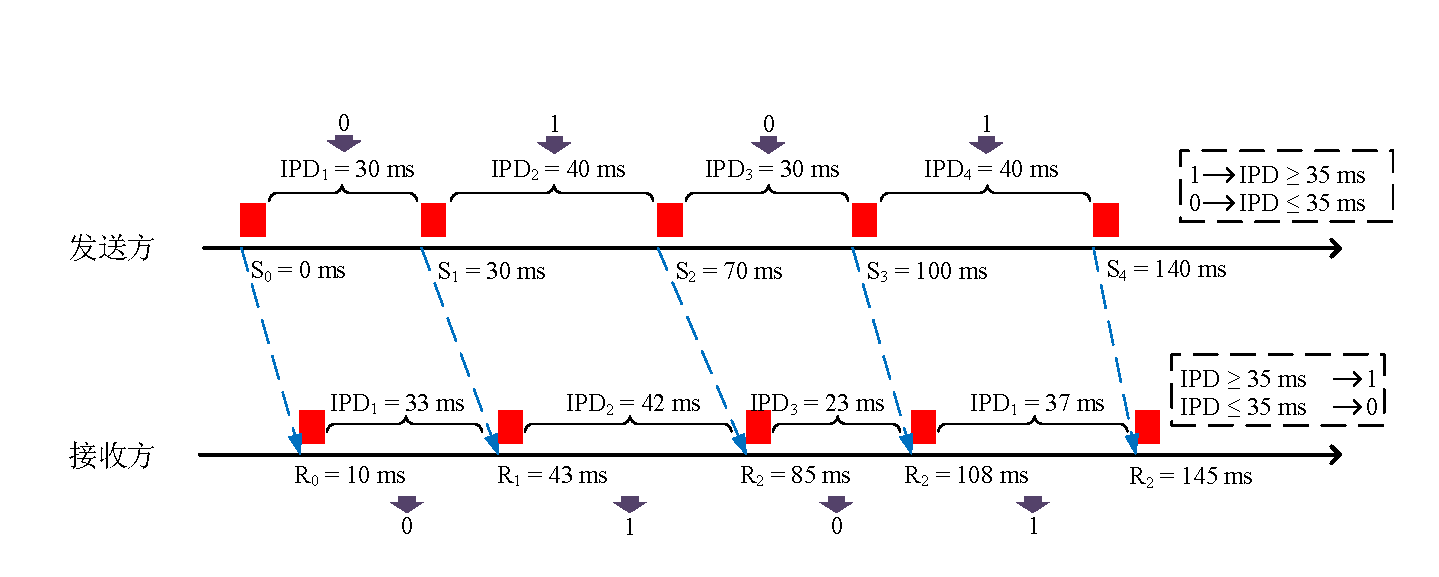
\includegraphics[width=0.99\textwidth]{chapters/chapter2/figures/ipd-ctc.pdf}
        \caption{基于IPD的时间隐通道示意图}\label{fig:2:ipd-ctc}
	\end{figure}
}

数据包传输过程存在时间间隔,利用该特征构建的时间隐通道,即为基于IPD的时间隐通道\nupcite{4317620,8600755,WALLS20111217}。如图\ \nref{fig:2:ipd-ctc},已知宿主信道的平均IPD为{35\ ms},待发送的二进制数据序列为$\{0,\ 1,\ 0,\ 1,\ \cdots\}$。对于发送方,当传输数据1时,将当前IPD调整为{35\ ms}以上;当传输数据0时,将当前IPD调整为{35\ ms}以内。图中根据数据包分布及消息内容,调整数据包发送时刻,实现隐通道调制。当数据包经网络传输后,噪声及传输调度导致IPD出现畸变。如果噪声太强,接收方接收的隐蔽消息将出现误码。

\insertFigure{ %on-off CTC
	\begin{figure}[htbp]
		\centering
        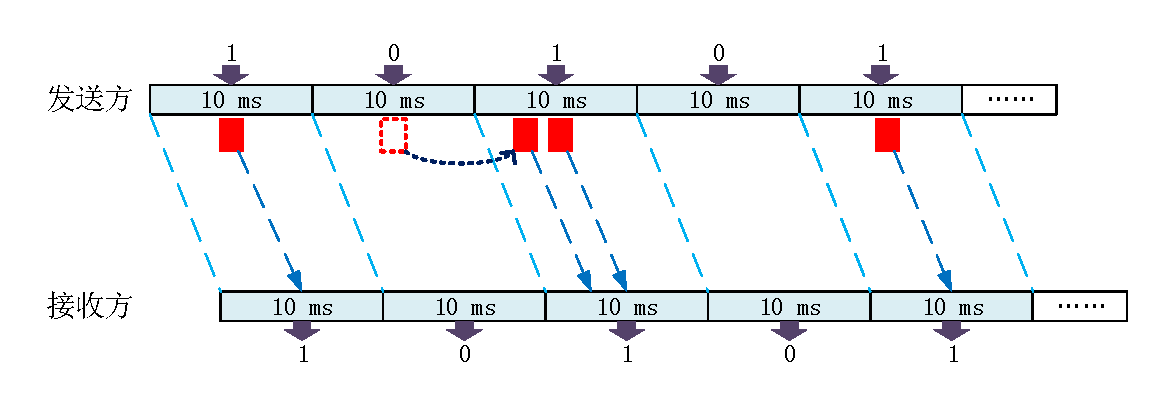
\includegraphics[width=0.9\textwidth]{chapters/chapter2/figures/onoff-ctc.pdf}
        \caption{基于On/Off模式的时间隐通道示意图}\label{fig:2:onoff-ctc}
	\end{figure}
}
另一种典型的时间隐通道为On/Off模式的时间隐通道,类似于开关的开关状态,通过控制是否传输数据包构建时间隐通道\nupcite{Cabuk:2004:ICT:1030083.1030108,5062145,6406084}。如图\ \nref{fig:2:onoff-ctc},发送方与接收方设定{10\ ms}的时间窗口,窗口内发送数据包则代表传输1,不发送则代表传输0。该类时间隐通道中,隐蔽消息编码适用不归零编码,双方利用时钟作为同步信号。

\insertFigure{ %Model-based CTC
	\begin{figure}[htbp]
		\centering
        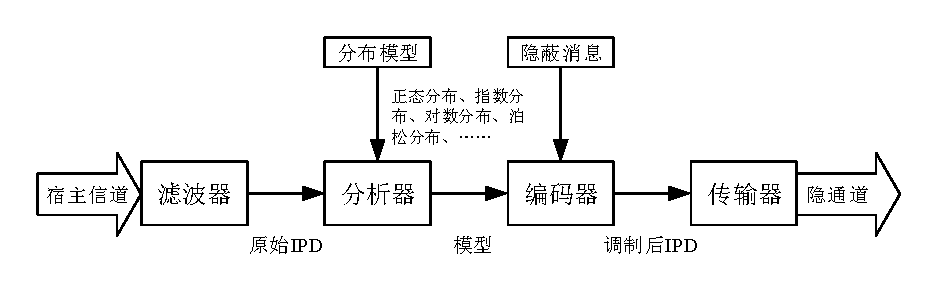
\includegraphics[width=0.85\textwidth]{chapters/chapter2/figures/mb-ctc.pdf}
        \caption{基于模型的时间隐通道示意图}\label{fig:2:mb-ctc}
	\end{figure}
}
基于模型的时间隐通道(MB-CTC),通过建模信道的传输特征,以分布拟合的方式提高抗检测能力。构建MB-CTC首先要对拟合目标建模,创建目标模型\nupcite{5062145,ahsan2002practical}。MB-CTC通常包含滤波器、分析器、编码器及传输器几个部分,实现隐通道调制。如图\ \nref{fig:2:mb-ctc},滤波器分析宿主信道的IPD特征,并将分析结果传送给分析器。分析器根据已知模型特征,判断当前适配的模型类型。编码器基于已知模型,参照概率分布函数及累积分布函数,将隐蔽消息编码进IPD。传输器根据目标IPD,调整数据包发送间隔,完成调制过程。

以太网环境中,数据包传输过程具有随机性及不确定性,时间隐通道对信道的影响有限,因此构建方法中对IPD等对象的修改空间较大。VoLTE通话时数据具有较明显的传输规律,因此对IPD及数据包顺序的大规模修改对隐蔽性影响较大,本文提出通过主动丢包的方式构建时间隐通道,通过模拟网络噪声导致的随机丢包事件,提高其抗检测能力。

\subsection{适于移动互联网的时间隐通道构建方法}
\label{chap:backinfo:ctc:mobile}
%介绍Skype、VoIP等构建方法
移动互联网环境下的时间隐通道构建方法,与以太网环境下时间隐通道的构建原理存在相似点。但移动互联网环境中,数据包传输特征不完全相同,适于以太网的时间隐通道构建方法在隐蔽性方面难以满足要求。

\insertFigure{
	\begin{figure}[htbp]
		\centering
        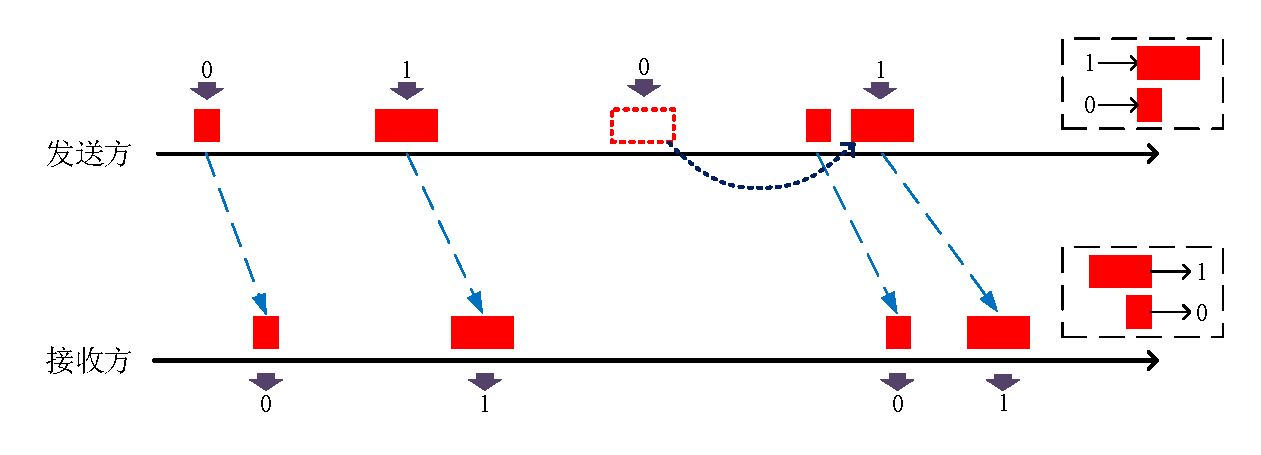
\includegraphics[width=0.95\textwidth]{chapters/chapter2/figures/pl-ctc.pdf}
        \caption{基于数据包长度的时间隐通道示意图}\label{fig:2:pl-ctc}
	\end{figure}
}

%Packet-Length CTC。 Liang
对于VoIP等实时交互应用,数据包长度并不完全随机,数据包长度与传输内容密切相关。构建基于数据包长度的时间隐通道,需要首先统计数据包长度分布,划分独立区间并与编码符号对应。发送过程中,根据数据包长度及当前消息内容,通过调整数据包顺序完成隐蔽消息嵌入\nupcite{LIANG2018144,8277839}。如图\ \nref{fig:2:pl-ctc},通过调整数据包队列,即可构建基于数据包长度的时间隐通道。

%Packet-content CTC
VoIP应用的RTP数据包,在一次通话中内容重复的几率较低。因此,数据包自身也构成了连续不断的特征流,并且数据包内容出现HASH碰撞的概率较低。基于数据包内容的时间隐通道借助信息摘要算法,以负载的摘要值为数据包特征。通过调整数据包顺序,构建数据包特征序列,实现隐通道构建\nupcite{LIANG2018162,6670985}。

%VoLTE RTP、RTCP CTC
由于VoLTE采用了基于RTP的传输方案,因此通过RTCP数据包实现传输反馈。由于同时存在两种数据包,发送序列中形成了数据包交叉。RTCP数据包数量较少,并且分布位置相对离散,具有切分数据包序列的功能。调整RTCP数据包之间的RTP数据包的数量,将隐蔽消息嵌入到RTP数据包数量中,即可构建时间隐通道\nupcite{ZHANG201866}。

\insertFigure{
	\begin{figure}[htbp]
		\centering
        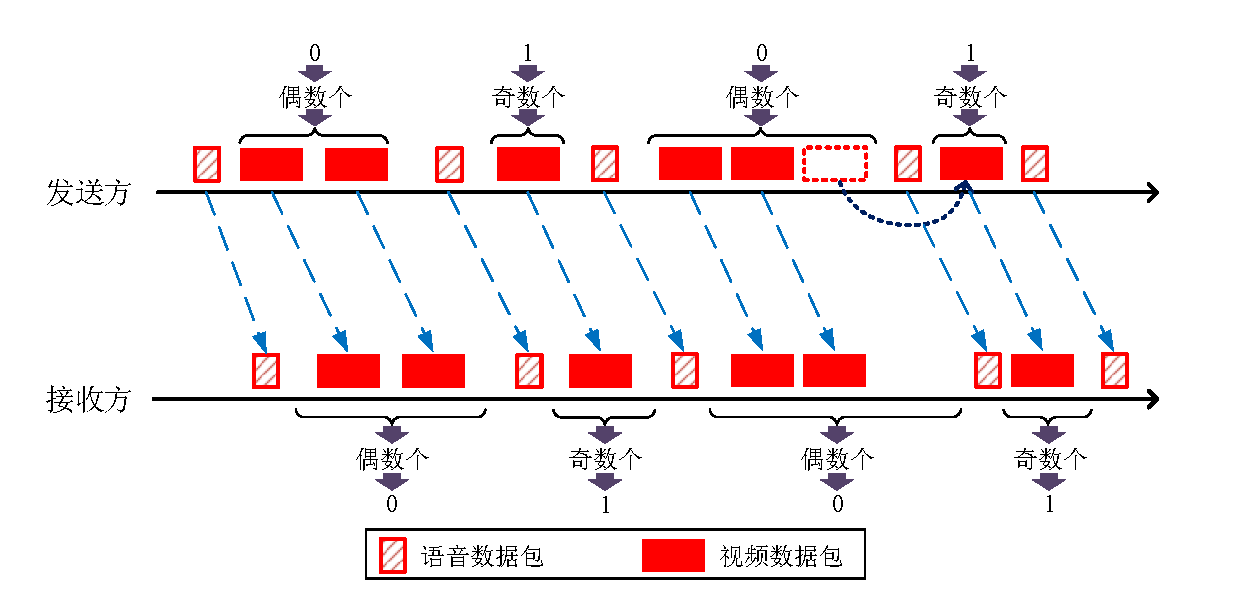
\includegraphics[width=0.9\textwidth]{chapters/chapter2/figures/av-ctc.pdf}
        \caption{基于数据包计数的时间隐通道示意图}\label{fig:2:av-ctc}
	\end{figure}
}

%VoLTE Video、Audio CTC
类似基于RTP及RTCP的时间隐通道\nupcite{ZHANG201866},基于语音数据包及视频数据包,根据数据包计数构建时间隐通道也是可行方法\nupcite{ZHANG201929}。由于语音数据包传输规律明确,因此与同步时钟具有相同功能。采用{AMR-WB(Adaptive Multi-Rate Wideband)}语音编码时,语音数据包每{20\ ms}发送一次。另一方面,视频帧率为{30\ fps}时的采样周期大约为{33\ ms},导致视频数据包与语音数据包的发送周期不同步。因此,调整语音数据包之间视频数据包数量,以视频数据包的数量表示隐蔽消息,能够构建时间隐通道。该模式的示意图如图\ \nref{fig:2:av-ctc},由于调整的数据包数量少,具有良好的隐蔽性。

适于移动互联网的时间隐通道构建方法,在结合应用特征的基础上,通常采用交换数据包的方式实现调制。本文提出通过主动丢包的方式构建时间隐通道,也是在VoLTE信道特征的基础上,通过模拟噪声的行为实现调制。

\subsection{时间隐通道的鲁棒性设计}
\label{chap:backinfo:ctc:robustness}
正如本文\ \nref{sec:intro:background:robustness}所述,时间隐通道在鲁棒性方面格外重视。隐通道常用的鲁棒性方法,包括鲁棒性编码、附加校验及纠错信息等。不同的方法各有优势,在应用中通常结合噪声类型,根据去噪需求确定鲁棒性策略。

%介绍各个方案中,为保证鲁棒性,采用的检错、纠错编码,重传策略等
%Gray码
\insertTable{
	\begin{table}[htbp]
        \centering
        \caption{格雷码编码表}
        \label{tab:2:gray-code}
        \begin{tabular*}{0.6\textwidth}{@{\extracolsep{\fill}}cccc}
        \toprule
        数据 & 1 bits格雷码 & 2 bits格雷码 & 3 bits格雷码\\ 
        \midrule
        0 & 0 & 00 & 000 \\ 
        1 & 1 & 01 & 001 \\ 
        2 &   & 11 & 011 \\ 
        3 &   & 10 & 010 \\ 
        4 &   &    & 110 \\ 
        5 &   &    & 111 \\ 
        6 &   &    & 101 \\ 
        7 &   &    & 100 \\ 
        \bottomrule
        \end{tabular*}
    \end{table}
}

\insertFigure{
	\begin{figure}[htbp]
		\centering
        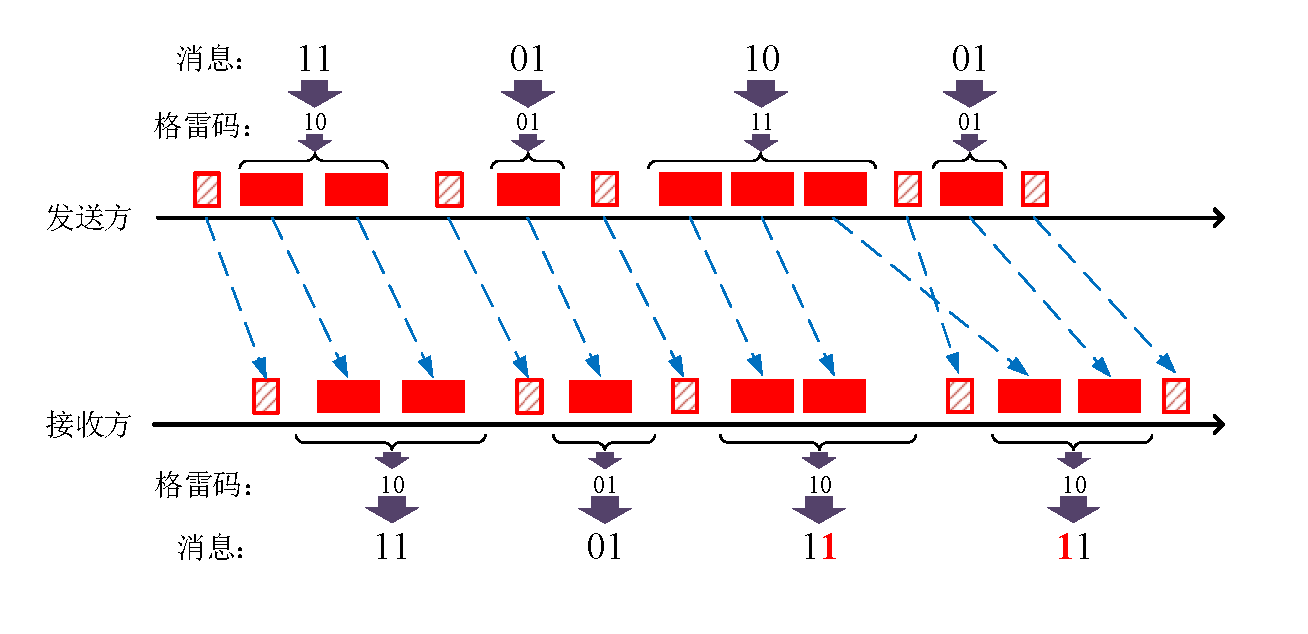
\includegraphics[width=0.9\textwidth]{chapters/chapter2/figures/gray-ctc.pdf}
        \caption{基于格雷码的时间隐通道鲁棒性示意图}\label{fig:2:gray-ctc}
	\end{figure}
}

格雷码又称循环二进制单位距离码,任意两个相邻数值的编码只有一个二进制位不同,与奇偶校验码同属于可靠性编码\nupcite{7329924}。格雷码编码如表\ \nref{tab:2:gray-code}所示,利用相邻数据编码差异小的优势,当噪声导致的错误只有$\pm1$时,误码只影响一个二进制位,降低了噪声导致的误码位数。格雷码的应用优势如图\ \nref{fig:2:gray-ctc},发送方通过数据包计数进行调制,接收过程中出现不可预期的乱序时,格雷码能够防止噪声扩散\nupcite{8600755,8817935}。

%Guard Band
受网络噪声的影响,编码符号之间的区分难度增大,需要在符号之间设定一定长度的隔离区,从而降低噪声干扰出错的几率。当符号落入隔离区时,则视为噪声丢弃,否则将产生误码。根据符号类型,隔离区通常设定为单个\nupcite{6567004,6296078},或多个\nupcite{LIANG2018162},与符号所表示的意义直接关联。

%喷泉码等
除以上方法外,一些特殊的编码算法,也应用在了时间隐通道中。基于喷泉码的时间隐通道,使用随机生成的关系矩阵,建立数据符号的线性编码。该方法保证了每个符号中有足够的冗余信息,结合抹除码的特征,在接收到足够的正确符号时,具有较好的保密性和鲁棒性\nupcite{6296078}。除了喷泉码,低密度奇偶校验码、里所码、卷积码、Turbo码均能在一定程度上提升鲁棒性\nupcite{10.1007/978-3-642-24178-9_22}。

时间隐通道的鲁棒性设计,与隐通道的信噪比相关联,从而具备极端情况下的传输能力。本文提出通过主动丢包的方式构建时间隐通道,离散的主动丢包与网络噪声在形式上具有一致性,因此对隐通道来说信噪比较低,鲁棒性方法需要对噪声进行有效识别。因此,基本的检错与纠错方法无法完全满足传输需求,需要利用不同阶段信噪比的差异,充分利用有限的传输资源。